\documentclass[a4paper,10pt,oneside]{book}

% packages 
\usepackage{arsclassica}    % fancy layout
\usepackage[english]{babel}\addto{\captionsenglish}{\renewcommand{\bibname}{References}}
\usepackage{caption}         % figure captions
\usepackage[square,numbers,super,sort&compress]{natbib}  % bibliography style
\usepackage[cc]{titlepic}    % enable logo on title page
\usepackage{graphicx}       % logo related

\usepackage{standalone}
\standalonetrue

% bibliography
\bibliographystyle{../thesis}

% title setup
\title{ \vspace{3in} Unravelling higher order genome organisation {\small [working
    title]} \\ \vspace{2em} {\large {\bf Results 5: Collaborations}} }
\author{Benjamin L. Moore}
\titlepic{\vspace{2.2in} 
\includegraphics[width=\textwidth]{/Users/benmoore/hvl/1yrReport/figs/igmm.png}}

\begin{document}

%\maketitle

\chapter{Local chromatin conformation}

\section{Introduction}

The Hi-C assay provides a genome-wide overview of chromatin conformation, however this broad scope imposes resolution limits inherent to an all-vs-all assay. For a closer look at chromatin conformation within a region of interest, alternative C-based assays such as 3C, 4C and 5C can be employed alongside classical microscopy techniques like FISH.

Here I discuss two collaborative projects involving the use of 4C-seq and 5C data to "zoom in" on two well-studied regions related to limb development: the ZRS enhancer and HoxD gene cluster.

\section{Chromatin conformation at the SHH locus}

\begin{figure}
\begin{center} 
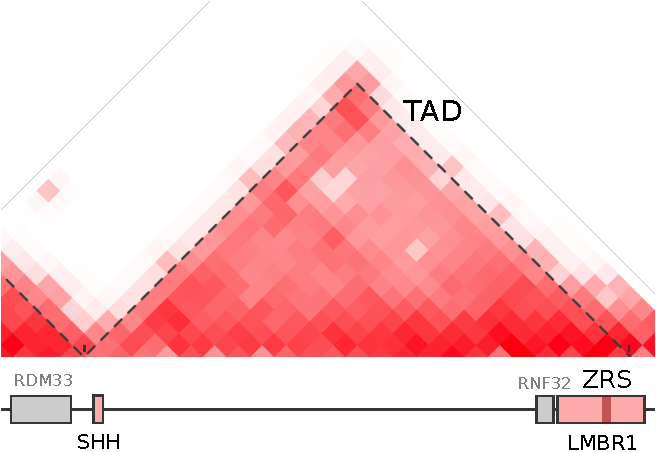
\includegraphics[width=.7\textwidth]{figs/shhtad.pdf}
\captionsetup{width=\textwidth} 
\caption[SHH--ZRS contacts occur within a stable TAD.]{ {\bf SHH--ZRS contacts occur within a stable TAD. }
An approximately 1 Mb region of the mouse genome is shown below a Hi-C contact map (derived from previously published data\cite{Dixon2012}). A clear TAD can be identified spanning from SHH to ZRS, dashed lines show TAD boundaries called by \citet{Dixon2012}. This figure was generated for \citet{Anderson2014a}.
}\label{fig:shhtad}
\end{center} 
\end{figure} 

Anterior-posterior patterning in the developing limb is regulated in mammals by \emph{Sonic hedgehog} (SHH).\cite{Anderson2012} Specifically, the SHH gene is expressed within a confined region named the "zone of polarising activity". Its expression within this region is known to be regulated by a well-studied enhancer, the "zone of polarising activity regulatory sequence" or ZRS.\cite{Hill2013a} ZRS is located almost 1 Mb downstream of its target SHH promoter in humans, and is located in intronic regions of another gene, LMBR1, and is conserved across mammals and fish (Fig. \ref{fig:shhtad}).\cite{Hill2013a, Laurell2012} Single point mutations and short insertions within this enhancer have been linked to various limb deformities, including pre- and post-axial polydactyly.\cite{Anderson2012, Lettice2008, Laurell2012} For example, a heritable point mutation in the ZRS enhancer is the cause of polydactyly in "Hemingway cats", a large group of domestic cats with extra toes that reside at the former home of Ernest Hemingway.\cite{Lettice2008}  

Collaborators have developed a model system which allows inducible SHH expression in a non-expressing cell line named 14fp. Application of trichostatin A (TSA) then leads to detectable SHH expression, and increased levels of the histone activation mark H3K27ac at the ZRS (\emph{unpublished data}). However, the question remains whether this TSA treatment is fundamentally altering local chromatin structure, that is, bring together the ZRS enhancer with its target SHH promoter, or whether ZRS and SHH are in contact in both the active and non-expressing cell lines and SHH expression is blocked through other means.

My part in this collaboration was to analyse 3C-seq (also known as 4C) data recorded by our collaboratoes for the SHH--ZRS region in mouse. Additionally, the 4C procedure was adapted for specific in-house sequencing instruments (Ion Torrent Ion Proton\textsuperscript{TM} sequenced as opposed to Illumina\textsuperscript{TM} technology) and as such required diagnostics to confirm the experimental data was accurate. 

% Adam sent a powerpoint he gave for section meeting, see also Prof Hill's publications

\subsection{Assay diagnostics}

\subsection{4C / Hi-C comparison}

\subsection{3D modelling with 5C data}

All-vs-all contacts either genome-wide in the case of Hi-C, or locally with 5C, can be used to infer the shape of chromatin fibres in three-dimensions through a variety of methods (e.g. \cite{Hu2013a, }).

\section{5C in the HoxD region}

HoxD is another well-studied genetic system involved in limb development and under the control of known enhancers.

% files for this under iain on ext HD
% relevant publications: http://dev.biologists.org/content/139/17/3157.full.pdf+html

%Iain's thesis: https://www.era.lib.ed.ac.uk/handle/1842/8056

\subsection{Differential contacts}

% raw diff: fold change?

\begin{figure}
\begin{center} 
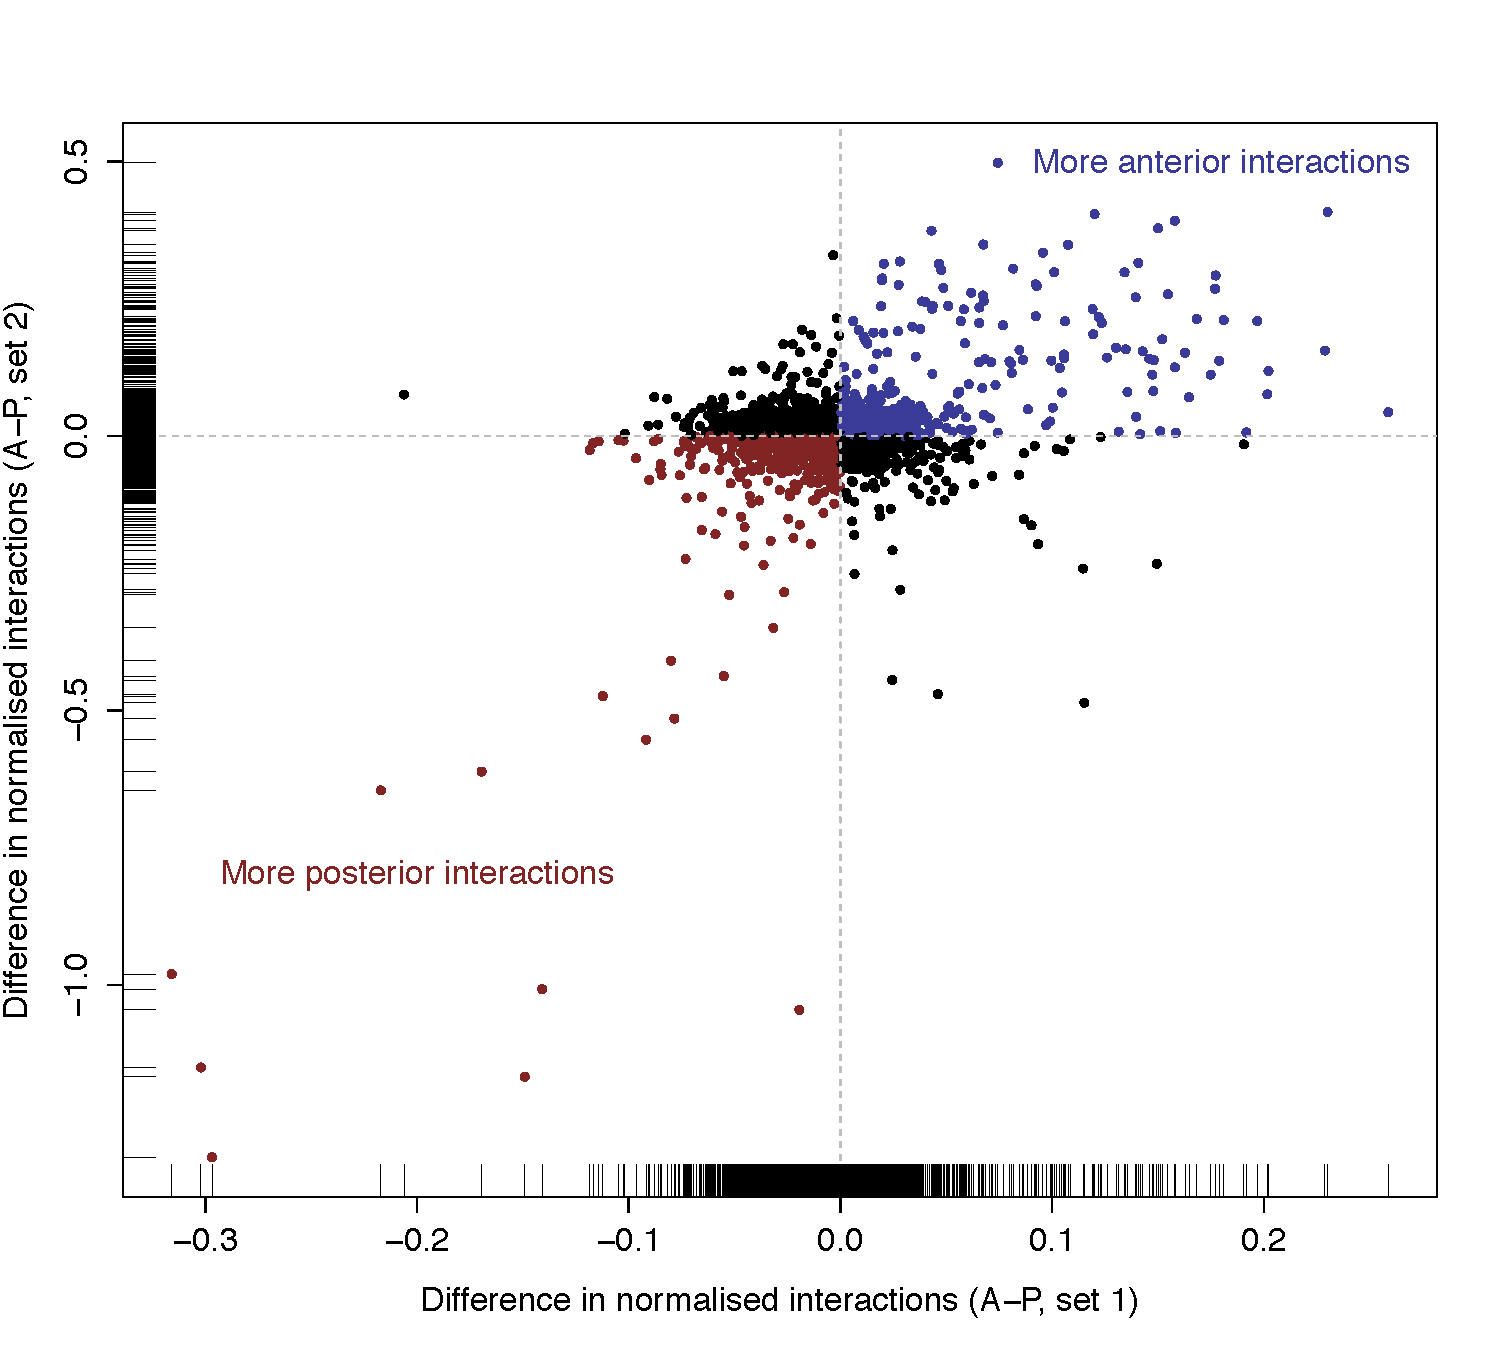
\includegraphics[width=\textwidth]{figs/5cfc.pdf}
\captionsetup{width=\textwidth} 
\caption{ {\bf Will we use this stuff? }
Placeholder
}\label{fig:5cfc}
\end{center} 
\end{figure} 

% statistical test of differential contacts

\begin{figure}
\begin{center} 
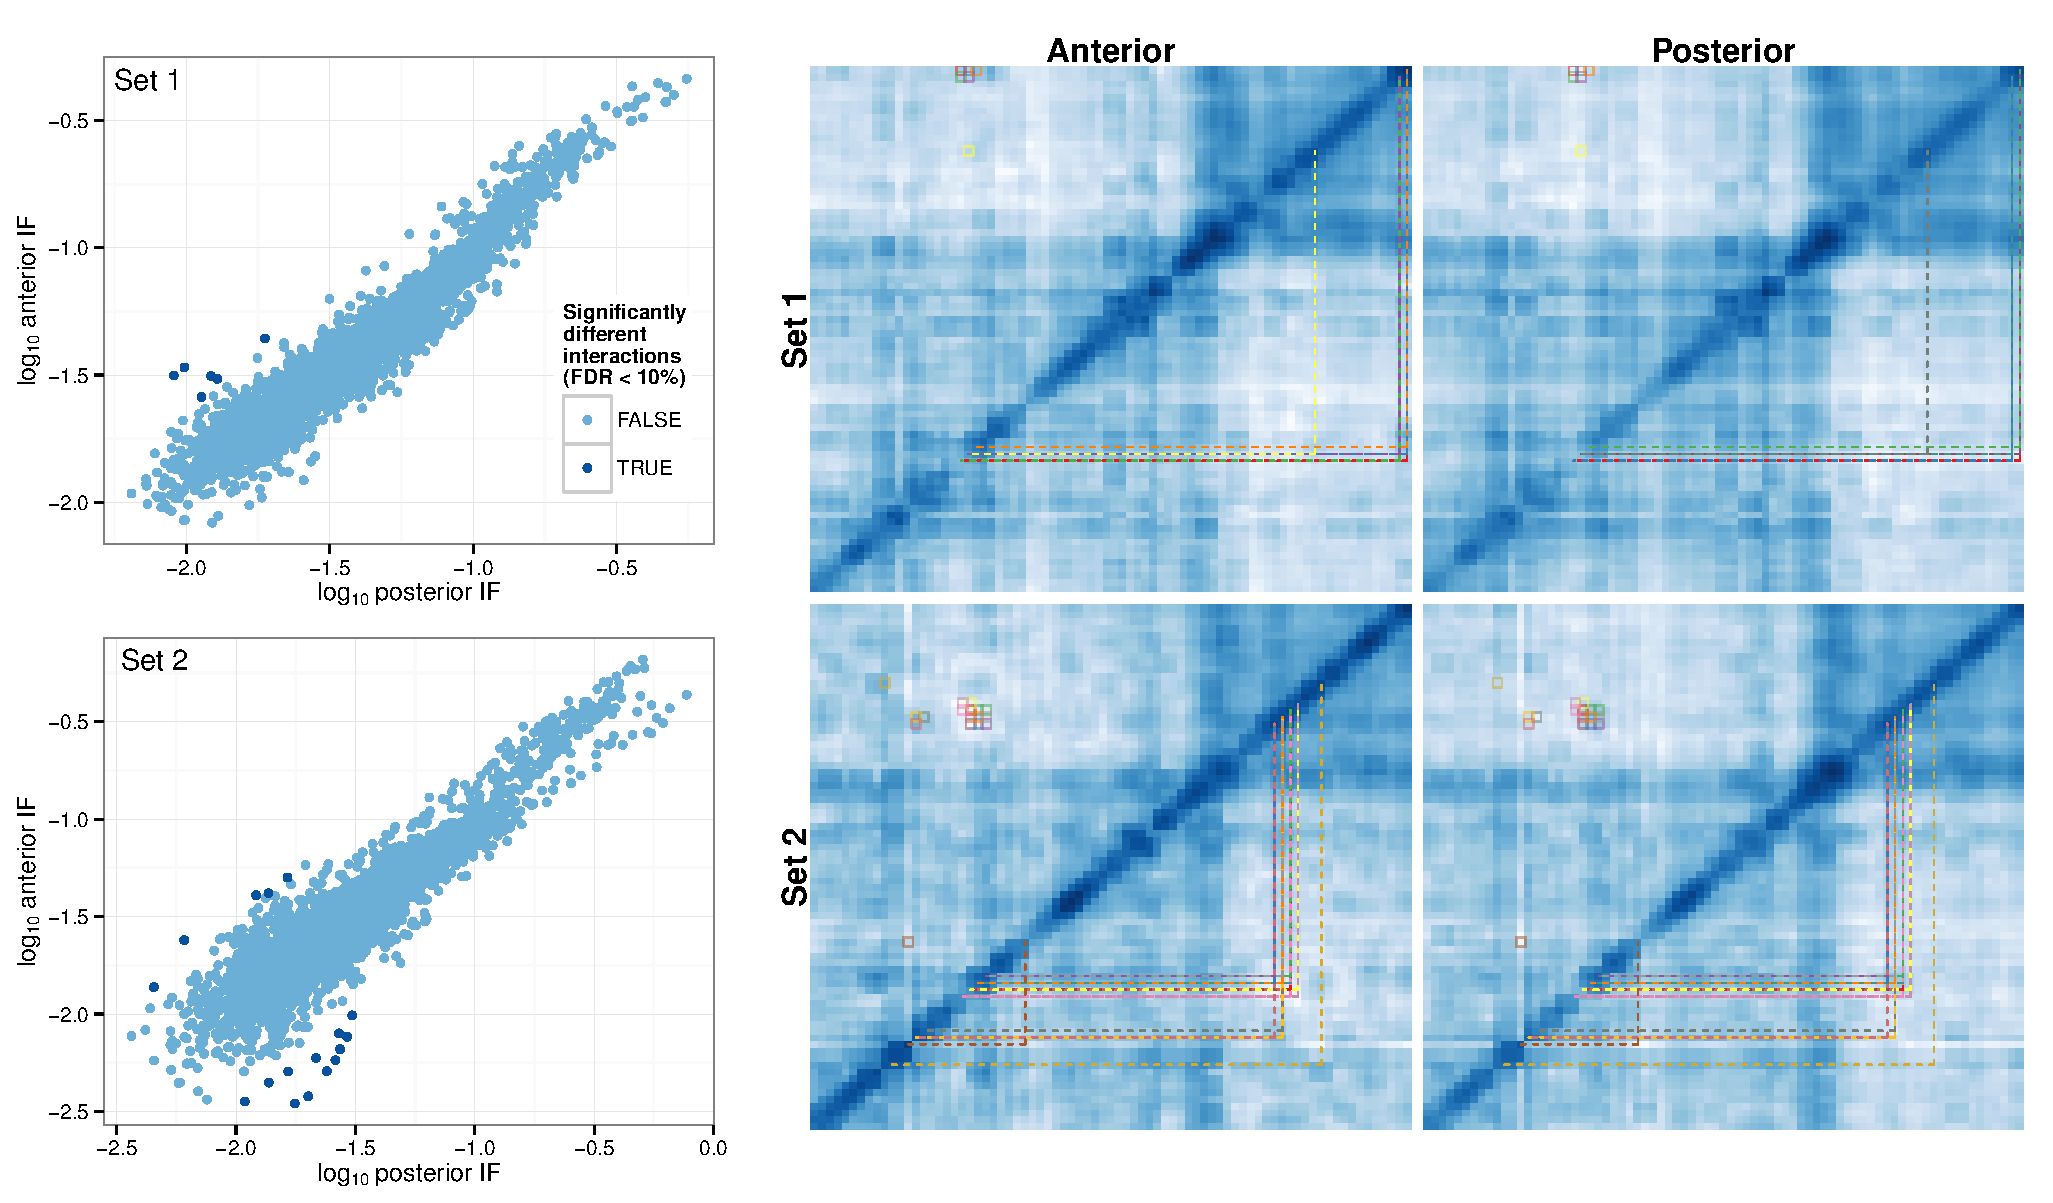
\includegraphics[width=\textwidth]{figs/5cdiff.pdf}
\captionsetup{width=\textwidth} 
\caption{ {\bf Will we use this stuff? }
Placeholder
}\label{fig:5cdiff}
\end{center} 
\end{figure} 


\subsection{5C / Hi-C comparison}

\begin{figure}
\begin{center} 
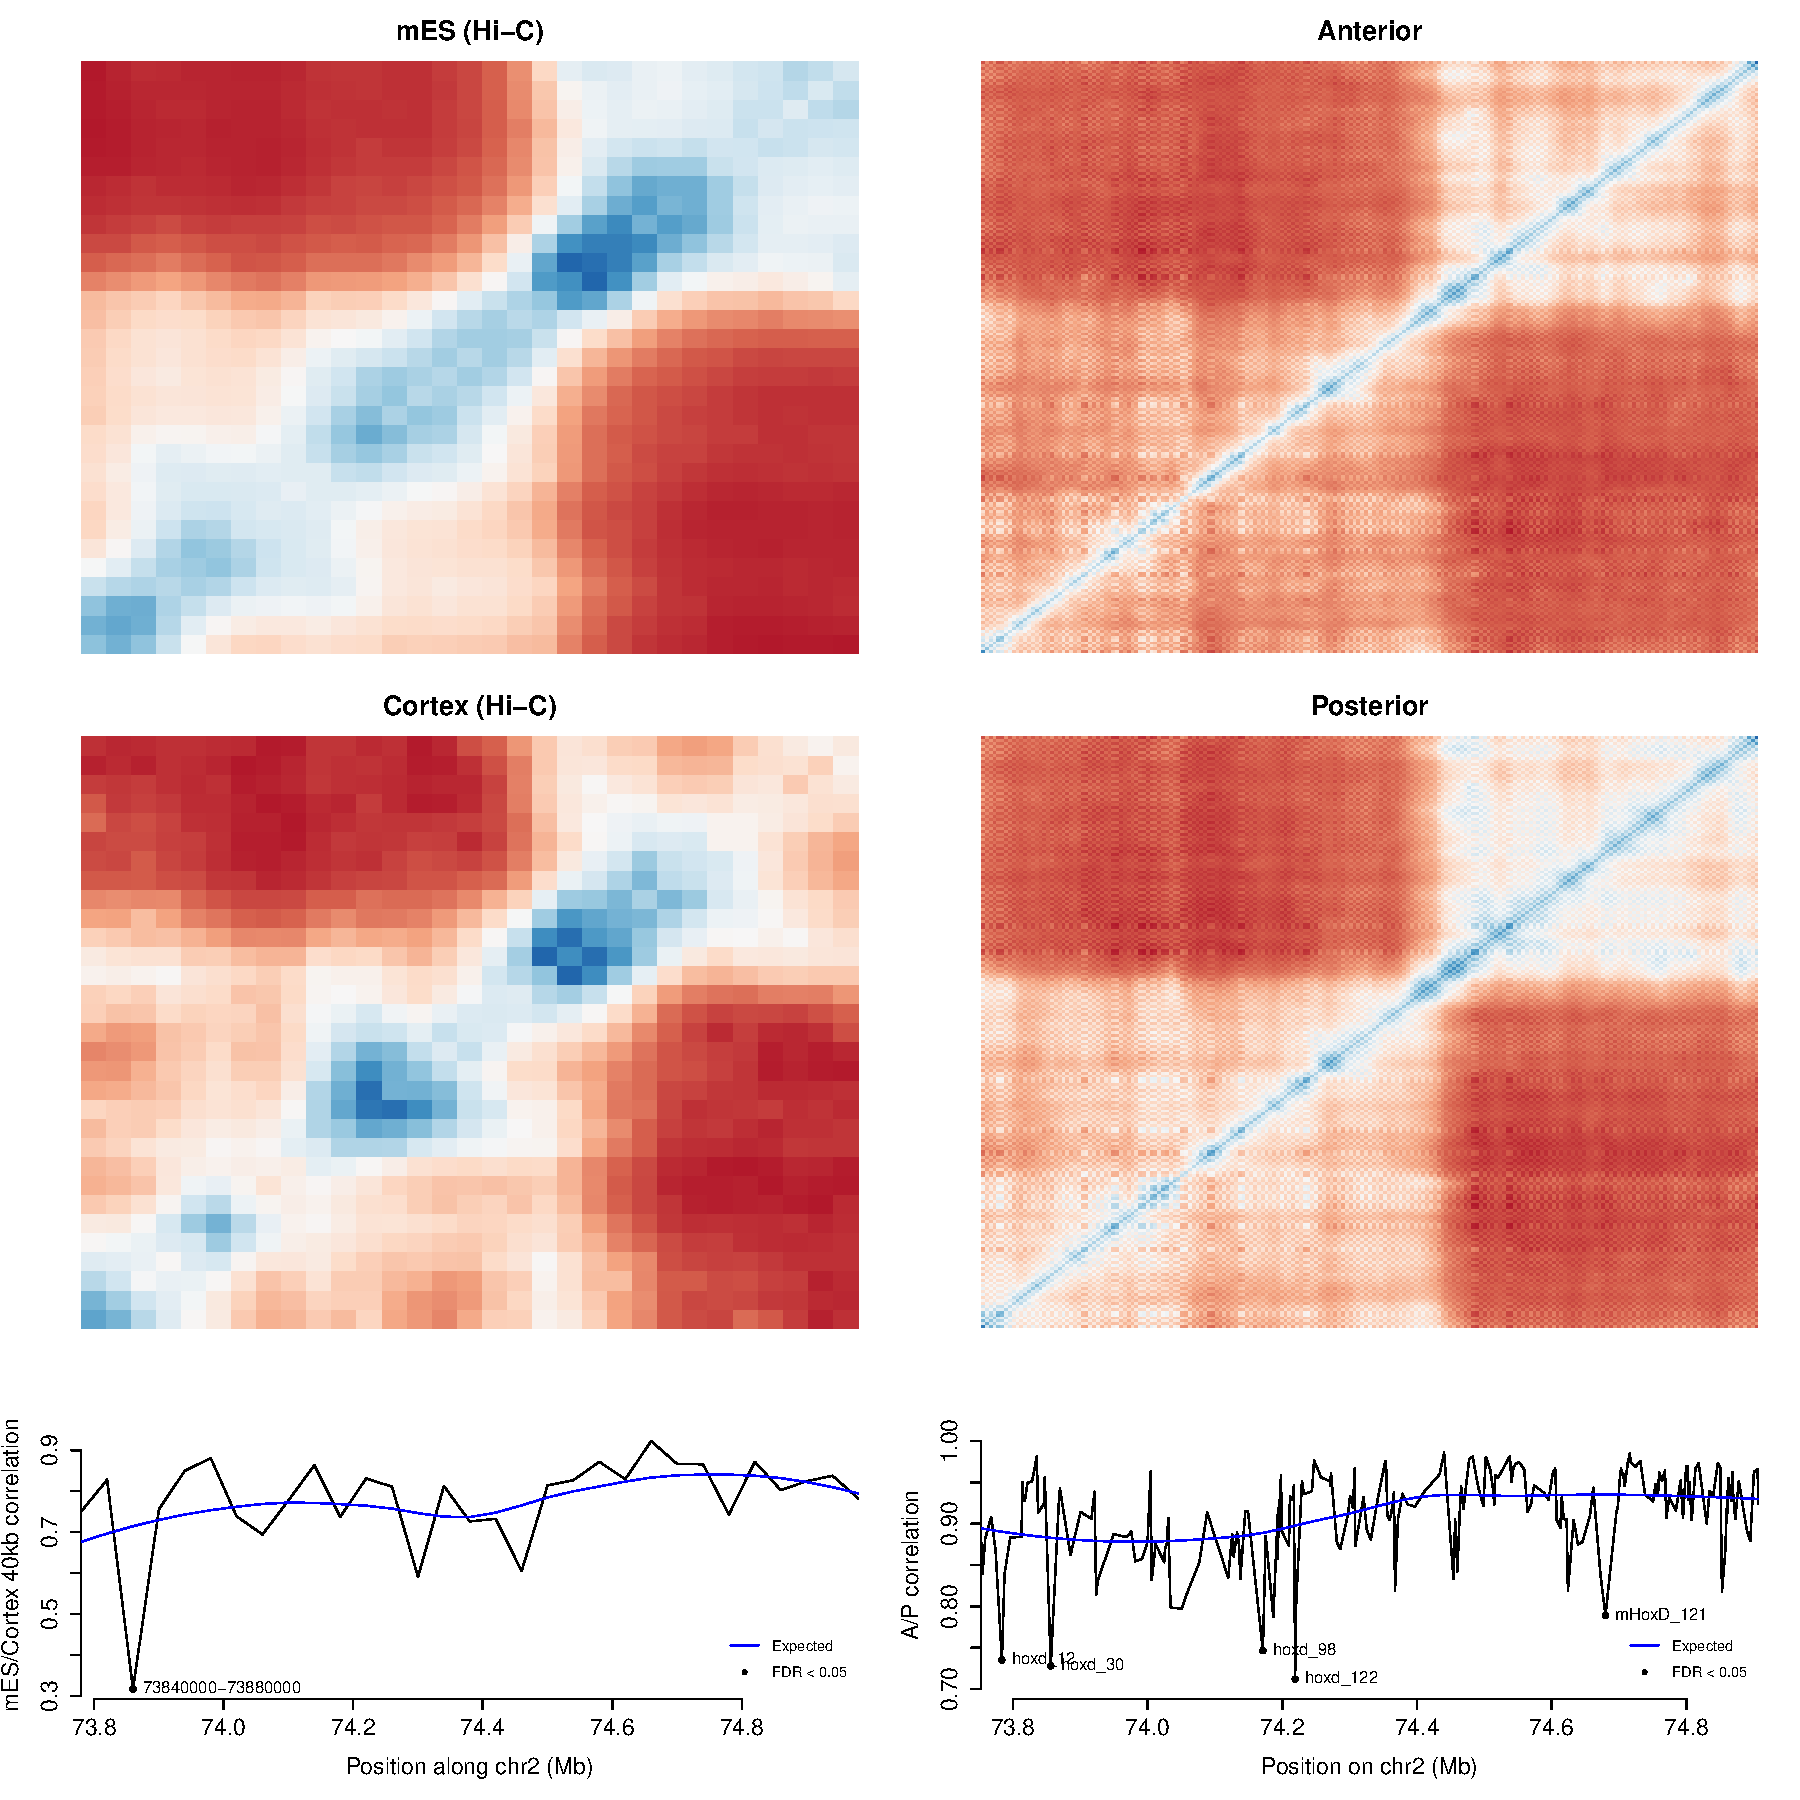
\includegraphics[width=\textwidth]{figs/5chic.pdf}
\captionsetup{width=\textwidth} 
\caption{ {\bf Will we use this stuff? }
Placeholder
}\label{fig:5cdiff}
\end{center} 
\end{figure} 


\ifstandalone
\begin{small}
\bibliography{/Users/benmoore/Documents/library,/Users/benmoore/Documents/customrefs}
\end{small}
\fi

\end{document}
